\documentclass[8pt,twocolumn]{article}

\usepackage[a4paper, margin=0.2in]{geometry}
\usepackage{titlesec}
\usepackage{enumitem}
\usepackage{amsmath}
\usepackage{hyperref}
\usepackage{graphicx}
\usepackage{tabularx}
\usepackage{xcolor}
\usepackage{setspace}
\usepackage{listings}  
\usepackage{dsfont}

\lstset{
  frame=tb,
  language=C,
  aboveskip=3mm,
  belowskip=3mm,
  showstringspaces=false,
  columns=flexible,
  basicstyle={\small\ttfamily},
  keywordstyle=\color{blue}\bfseries,       % <<<< keyword styling
  commentstyle=\color{gray}\itshape,
  stringstyle=\color{orange},
  numbers=none,
  breaklines=true,
  breakatwhitespace=true,
  tabsize=3,
  % If you want to highlight extra words:
  morekeywords={uint32_t,size_t,shmat,shmget, sem_t, sem_wait, sem_post, SharedMem} % add your own identifiers here
}
\setstretch{0.2}
\setlength{\extrarowheight}{0pt}
\setlength{\parskip}{0pt}
\begin{document}
\begin{itemize}[leftmargin=2em]
    \setlength{\itemsep}{0pt} % No extra space between items
    \setlength{\parskip}{0pt}
    \item The child process from \texttt{fork()} receives a copy-on-write duplicate of the parent's memory and file descriptor table.
    \item Use \texttt{wait()} or \texttt{waitpid()} in the parent to reap the child and avoid zombie processes.
    \item Each child should call \texttt{exit()} (or return from \texttt{main()}) to terminate cleanly.
    \item All \texttt{exec*()} functions replace the current process image with a new program.
\end{itemize}
\begin{center}
\vspace{-1.0em}
\resizebox{\linewidth}{!}{
    \vspace{1em} % Small vertical gap between the two tables
    \begin{tabular}{|l|l|c|c|}
      \hline
      \textbf{Function} & \textbf{Arguments} & \textbf{PATH} & \textbf{Custom Env} \\
      \hline
      \texttt{execl(path, arg0, …, NULL)}    & Arg list, full path            & No  & No  \\
      \hline
      \texttt{execlp(file, arg0, …, NULL)}   & Arg list, search \texttt{PATH} & Yes & No  \\
      \hline
      \texttt{execle(path, arg0, …, NULL, envp)} & Arg list, full path        & No  & Yes \\
      \hline
      \texttt{execv(path, argv[])}           & Arg vector, full path         & No  & No  \\
      \hline
      \texttt{execvp(file, argv[])}          & Arg vector, search \texttt{PATH} & Yes & No  \\
      \hline
      \texttt{execvpe(file, argv[], envp[])} & Arg vector, \texttt{PATH}, env  & Yes & Yes \\
      \hline
      \end{tabular}
}
  
\vspace{-0.6em}
\end{center}
\begin{itemize}[leftmargin=2em]
    \setlength{\itemsep}{0pt} % No extra space between items
    \setlength{\parskip}{0pt}
    \item \texttt{pthread\_create(\\ pthread\_t *thread, const pthread\_attr\_t *attr, void *(*start\_routine)(void *), void *arg)} \\
    Spawns a thread that shares the same address space. Returns \texttt{0} on success.

    \item \texttt{pthread\_join(pthread\_t thread, void **retval)} \\
    Waits for a thread to finish and optionally retrieves its return value. Returns \texttt{0} on success.

    \item \texttt{pthread\_exit(void *retval)} \\
    Terminates the calling thread and makes \texttt{retval} available to \texttt{pthread\_join()}. Does not return.
    \item Semaphores (\texttt{sem\_t}) are integer counters used to control access to shared resources.
    \item \texttt{sem\_init(sem, [0(thread)|1(process)], value)} — Initialize semaphore to given value.
    \item \texttt{sem\_wait(sem)} — Decrement; blocks if value is 0.
    \item \texttt{sem\_post(sem)} — Increment; unblocks one waiter if any.
    \item \texttt{sem\_destroy(sem)} — Cleans up; does not free memory.
    \item Used for mutual exclusion (binary semaphores) or limiting access (counting semaphores).
\end{itemize}
\vspace{-0.6em}
\textbf{Dining Philosophers: Limit-Seat Strategy}
\vspace{-0.6em}
\begin{itemize}
    \setlength{\itemsep}{0pt} % No extra space between items
    \setlength{\parskip}{0pt}
    \item Using a semaphore initialized to \( N - 1 \) prevents deadlock in the dining philosopher problem.
    \item Limits the number of philosophers who can attempt to pick up chopsticks to ensure progress.
    \item Prevents circular wait, breaking one of Coffman’s deadlock conditions.
    \item Starvation is still possible due to unfair scheduling.
\vspace{-0.6em}
\begin{lstlisting}
typedef struct {
    int _status[N];
    sem_t mutex;
    sem_t sem[N]; 
} SharedMem;
void takeChpStk(SharedMem* shm, int i) 
    sem_wait(&shm->mutex);
    shm->_status[i] = HUNGRY;
    safeToEat(shm, i);
    sem_post(&shm->mutex);
    sem_wait(&shm->sem[i]);            
void safeToEat(SharedMem* shm, int i) 
    if ((shm->_status[i] == HUNGRY) &&
        (shm->_status[LEFT] != EATING) &&
        (shm->_status[RIGHT] != EATING)) {
            shm->_status[i] = EATING;
            sem_post(&shm->sem[i]);} 
void putChpStk(SharedMem* shm, int i) 
    sem_wait(&shm->mutex);
    shm->_status[i] = THINKING;
    safeToEat(shm, LEFT);
    safeToEat(shm, RIGHT);
    sem_post(&shm->mutex);            
\end{lstlisting}
\vspace{-1.5em}
\end{itemize}
\begin{itemize}
    \setlength{\itemsep}{0pt} % No extra space between items
    \setlength{\parskip}{0pt}
    \item \textbf{Turnaround t}: Total time from job arrival to completion.
    \item \textbf{Response t}: Time from job arrival to first CPU execution.
    \item \textbf{Waiting time}: Time a job spends in the ready queue.
    \item \textbf{Throughput}: Number of jobs completed per unit time.
\end{itemize}
\vspace{-0.6em}
\resizebox{\linewidth}{!}{%
\begin{tabular}{|l|c|c|c|c|c|}
\hline
\textbf{Algorithm} & \textbf{Preemptive} & \textbf{Fairness} & \textbf{Resp T} & \textbf{Turarnd T} & \textbf{Starv} \\
\hline
FCFS    & No       & by order               & $\downarrow$                        & $\uparrow$ (convoy effect)       & $\downarrow$ \\
\hline
SJF     & No       & No                               & $\uparrow$ short jobs    & Optm (theo)      & $\uparrow$ \\
\hline
SRT     & Yes      & No                               & $\uparrow$ short jobs         & Optm                    & $\uparrow$ \\
\hline
RR      & Yes      & Yes                              & $\uparrow$                        & dep (qtm)& Low \\
\hline
Lottery & Can &                     & $\tilde{\text{Fair}}$             & $\tilde{\text{Fair}}$            & $\downarrow$ \\
\hline
MLFQ    & Yes      & Adaptive                         & $\uparrow$                   & Adaptive                   & dep \\
\hline
\end{tabular}%
}

\textbf{Table storage:}
\vspace*{-0.8em}
\begin{itemize}
    \setlength{\itemsep}{0pt} % No extra space between items
    \setlength{\parskip}{0pt}
    \item UPP: user process pages
    \item SWAP: Non-memory resident iser process page 
    \item Process page table: in PCB table in OS mem region in RAM
    \item Open file table: in OS mem region in RAM
    \item File descriptor table: in PCB 
    \item Dynamically allocated mem in a prgram: UPP or SWAP
    \item file decriptor returned from an open(...) syscall: UPP or SWAP
    \item compiled binary files: not part of the virtual mem
\end{itemize}
\vspace{-0.6em}
\textbf{Contiguous mem:}
\vspace{-0.6em}
\begin{itemize}
    \setlength{\itemsep}{0pt} % No extra space between items
    \setlength{\parskip}{0pt}
  \item \textbf{Tracking free space:}
\vspace{-0.6em}
  \begin{itemize}
    \setlength{\itemsep}{0pt} % No extra space between items
    \setlength{\parskip}{0pt}
    \item Bitmap: 1 bit per block, where 0 = free, 1 = allocated.
    \item Linked List: Each free block links to the next.
    \item Buddy System: Memory is split into power-of-2 blocks; recursive splitting/merging.
  \end{itemize}
\vspace{-0.6em}
  \item \textbf{Fragmentation:}
\vspace{-0.6em}
  \begin{itemize}
    \setlength{\itemsep}{0pt} % No extra space between items
    \setlength{\parskip}{0pt}
    \item Internal: Block larger than needed.
    \item External: Gaps between allocated blocks.
  \end{itemize}
\vspace{-0.6em}
\end{itemize}
\vspace{-0.6em}
\textbf{Paging}
\vspace{-0.6em}
\begin{itemize}
    \setlength{\itemsep}{0pt} % No extra space between items
    \setlength{\parskip}{0pt}
  \item Fixed-size units: Logical pages and physical frames.
  \item Page Table: Maps pages to frames.
  \item TLB: Hardware cache for recent page table entries.
\end{itemize}
\vspace{-0.6em}
\textbf{Segmentation}
\vspace{-0.6em}
\begin{itemize}
    \setlength{\itemsep}{0pt} % No extra space between items
    \setlength{\parskip}{0pt}
  \item Logical memory divided into named segments (code, stack, heap).
  \item Each has a base and limit.
  \item Logical Address = \texttt{<Segment ID, Offset>}.
\end{itemize}
\vspace{-0.6em}
\textbf{Virtual mem}
\vspace{-0.6em}
\begin{itemize}
    \setlength{\itemsep}{0pt} % No extra space between items
    \setlength{\parskip}{0pt}
  \item Logical memory can exceed physical memory.
  \item Disk serves as backing store.
\end{itemize}
\vspace{-0.6em}
\textbf{Demand Paging}
\vspace{-0.6em}
\begin{itemize}
    \setlength{\itemsep}{0pt} % No extra space between items
    \setlength{\parskip}{0pt}
  \item Pages are only loaded on access. No memory resident page 
  \item (+) Reduces startup time and memory usage.
  \item (-) more page fault at start; page fault can cascade on other processes (e.g. thrashing)
\end{itemize}
\vspace{-0.6em}
\textbf{Page Access}
\vspace{-0.6em}
\begin{lstlisting}
    Check page table:
        if memory resident: acess physical mem; done;
        else: [page fault] -> trap to OS
            locate page in secondary storage;
            load into physical mem;
            update page table;
            goto Check page table;
\end{lstlisting}
\vspace{-0.6em}
\textbf{Single-Level Direct paging}
\vspace{-0.6em}
\begin{itemize}
    \setlength{\itemsep}{0pt} % No extra space between items
    \setlength{\parskip}{0pt}
  \item Flat array of entries.
  \item Wasteful for sparse address spaces.
\end{itemize}
\vspace{-0.6em}
\textbf{Multilevel}
\vspace{-0.6em}
\begin{itemize}
    \setlength{\itemsep}{0pt} % No extra space between items
    \setlength{\parskip}{0pt}
  \item Use a page directory pointing to page tables.
  \item Only allocate when needed.
  \item page dir base reg \texttt{$\rightarrow<$page\_dir\#, page\#, ofst$>$}
  \item overhead = sizeof(page\_dir) + $\sum$sizeof(small\_pagetable)
\end{itemize}
\vspace{-0.6em}
\textbf{Inverted Page Table}
\vspace{-0.6em}
\begin{itemize}
    \setlength{\itemsep}{0pt} % No extra space between items
    \setlength{\parskip}{0pt}
  \item One entry per frame: \texttt{<pid, page\#>} $\rightarrow$ frame.
  \item Compact but slow due to full-table lookup.
\end{itemize}
\vspace{-0.6em}
\textbf{Temporal Locality:} Recently used memory will be used again.\\
\textbf{Spatial Locality:} Nearby memory addresses are likely to be used soon.
\vspace{-1.0em}
\subsection*{Page Replacement Algorithms}
\vspace{-0.6em}
\begin{itemize}
    \setlength{\itemsep}{0pt} % No extra space between items
    \setlength{\parskip}{0pt}
  \item OPT: Replace page with furthest next use (ideal).
  \item FIFO: Oldest page out.
  \item LRU: Least recently used page.
  \item Clock: Approximate LRU using reference bits.
\end{itemize}
\vspace{-1.0em}
\[
T_{access} = (1 - p) \cdot T_{mem} + p \cdot T_{page\_fault}
\]
\textbf{Local Replacement}
\vspace{-1.0em}
\begin{itemize}
    \setlength{\itemsep}{0pt} % No extra space between items
    \setlength{\parskip}{0pt}
  \item Only evict pages from the same process.
  \item Predictable and isolated.
  \item if not enf allocated, hinders process progress
\end{itemize}
\vspace{-0.6em}
\textbf{Global Replacement}
\vspace{-0.6em}
\begin{itemize}
    \setlength{\itemsep}{0pt} % No extra space between items
    \setlength{\parskip}{0pt}
  \item Victim page can belong to any process.
  \item More flexible, allows self-adjustment, but less stable.
  \item bad behaved process can affect others
\end{itemize}
\vspace{-0.6em}
\textbf{Thrashing}
\vspace{-0.6em}
\begin{itemize}
    \setlength{\itemsep}{0pt} % No extra space between items
    \setlength{\parskip}{0pt}
  \item Excessive page faults reduce CPU utilization.
  \item Can lead to cascading faults in global replacement.
  \item \textbf{Working Set Model:} Allocate enf frames for \texttt{W(t, $\Delta$)}.
\end{itemize}
\begin{itemize}
    \setlength{\itemsep}{0pt} % No extra space between items
    \setlength{\parskip}{0pt}
    \item A file is the smallest amount of information that can be written to secondary memory.
    It is a named collection of data, used for organizing secondary memory
    \item A file type is a description of the information contained in the file. A file extension is
    a part of the file name that follows a dot and identifies the file type
    \item What does it mean to open and close a file?
Operating systems keep a table of currently open files. The open operation enters the
file into this table and places the file pointer at the beginning of the file. The close
operation removes the file from the table of open files.
    \item Truncating a file means that all the information on the file is erased but the
    administrative entries remain in the file tables. Occasionally, the truncate operation
    removes the information from the file pointer to the end.
\end{itemize}
\begin{table}[h!]
    \centering
    \renewcommand{\arraystretch}{0.6}
    \begin{tabular}{|l|p{6cm}|}
    \hline
    \textbf{Aspect} & \textbf{Memory Management} \\
    \hline
    Underlying Storage & RAM \\
    \hline
    Access Speed & Constant \\
    \hline
    Unit of Addressing & Physical memory address \\
    \hline
    Usage & Address space for process \newline \textbf{Implicit} when process runs \\
    \hline
    Organization & \textbf{Paging/Segmentation}: determined by HW \& OS \\
    \hline
    \end{tabular}
    \end{table}

    \begin{table}[h!]
        \centering
        \renewcommand{\arraystretch}{0.6}
        \begin{tabular}{|l|p{6cm}|}
        \hline
        \textbf{Aspect} & \textbf{File System Management} \\
        \hline
        Underlying Storage & Disk \\
        \hline
        Access Speed & Variable disk I/O time \\
        \hline
        Unit of Addressing & Disk sector \\
        \hline
        Usage & Non-volatile data \newline \textbf{Explicit} access \\
        \hline
        Organization & \textbf{Many FS types}: ext* (Linux), FAT* (Windows), HFS* (Mac) \\
        \hline
        \end{tabular}
        \end{table}
        \vspace{-1.5em} % Small vertical gap between the two tables
\begin{itemize}
    \setlength{\itemsep}{0pt} % No extra space between items
    \setlength{\parskip}{0pt}
  \item \textbf{Name}: A human-readable reference to the file.
  \item \textbf{Identifier}: A unique ID for the file used internally by the file system.
  \item \textbf{Type}: Indicates the type of file (e.g., executable, text file, object file, directory, etc.).
  \item \textbf{Size}: Current size of the file (in bytes, words, or blocks).
  \item \textbf{Protection}: Access permissions, which may include reading, writing, and execution rights.
  \item \textbf{Time, date, and owner information}: Includes creation time, last modification time, owner ID, etc.
  \item \textbf{Table of content}: Metadata that enables the file system to determine how to access the file.
\end{itemize}
\vspace*{-1.2em}
\begin{itemize}
    \setlength{\itemsep}{0pt} % No extra space between items
    \setlength{\parskip}{0pt}
    \item A process uses the \texttt{open()} system call to access a file:
      \item Updates the process’s \textbf{Per-Process File Descriptor Table}: \texttt{fd} points to the corresponding system-wide table entry.
    \item Shared file descriptors:
\vspace{-0.6em}
    \begin{itemize}
        \setlength{\itemsep}{0pt} % No extra space between items
        \setlength{\parskip}{0pt}
      \item Two \texttt{fd}s pointing to the same system-wide entry share offset and metadata.
      \item Created using \texttt{dup/2()}, or inherited from \texttt{fork()}.
    \end{itemize}
\vspace{-0.6em}
  \end{itemize}
\vspace{-1.5em}

  \begin{table}[ht]
    \centering
    \resizebox{\linewidth}{!}{
    \begin{tabular}{|l|c|c|c|c|}
    \hline
    \textbf{Feature} & \textbf{Contiguous} & \textbf{Linked List} & \textbf{FAT} & \textbf{Inode-based (e.g., ext)} \\
    \hline
    Access time (random) & Fast & Slow & Moderate & Fast \\
    Access time (sequential) & Fast & Fast & Fast & Fast \\
    Disk fragmentation & High & None & None & Low \\
    Supports random access & Yes & No & Yes (with FAT table) & Yes \\
    Space efficiency & Poor & Good & Good & Very good \\
    Pointer overhead & None & High & High (FAT in memory) & Low (indirect blocks) \\
    File size flexibility & Poor & Good & Good & Excellent \\
    Crash recovery & Poor & Poor & Moderate & Good (journaling) \\
    \hline
    \end{tabular}
    }
    \end{table}

\vspace{-1.5em}
        \begin{table}[ht]
\centering
\resizebox{\linewidth}{!}{
\begin{tabular}{|l|c|c|c|}
\hline
\textbf{Feature} & \textbf{FAT} & \textbf{EXT (inode)} & \textbf{NTFS (MFT)} \\
\hline
Allocation method & FAT table (linked list) & Inode + indirect blocks & Extents + B-tree indexing \\
Metadata location & Centralized table & Distributed inodes & MFT entries \\
Scalability & Poor for large disks & Very scalable & Highly scalable \\
Crash tolerance & Low (no journaling) & High (journaling via ext3/4) & High (journaling) \\
Maximum file size & Limited & Large (ext4: 16 TiB) & Very large \\
Directory management & Linear list & Hash tree (ext4) & B-tree \\
\hline
\end{tabular}
}
\end{table}
\centering
\resizebox{\linewidth}{!}{
  \begin{tabular}{|l|c|c|}
  \hline
  \textbf{Feature} & \textbf{Hard Link} & \textbf{Symbolic Link} \\
  \hline
  Points to & Inode (actual file) & File path (string) \\
  Requires own inode & No & Yes \\
  Spans file systems & No & Yes \\
  Can link to directory & No & Yes \\
  Broken if target deleted & No & Yes (becomes dangling) \\
  Deletes actual file? & Only if last hard link removed & No \\
  ls -l output & Normal file & l with → path \\
  \hline
  \end{tabular}
}
\vspace{-0.6em}
\begin{itemize}
  \setlength{\itemsep}{0pt} % No extra space between items
  \setlength{\parskip}{0pt}
  \item \textbf{\texttt{open(const char *pathname, int flags[,mode])}}:
\vspace{-0.6em}
    \begin{itemize}
      \setlength{\itemsep}{0pt} % No extra space between items
      \setlength{\parskip}{0pt}
      \item Opens a file and returns a file descriptor (int).
      \item \texttt{flags}: \texttt{O\_RDONLY}, \texttt{O\_WRONLY}, \texttt{O\_RDWR}, \texttt{O\_CREAT}, etc.
      \item \texttt{mode} required if \texttt{O\_CREAT} is used, set permission bits.
    \end{itemize}
\vspace{-0.6em}
  \item \textbf{\texttt{read(int fd, void *buf, size\_t count)}}:
\vspace{-0.6em}
    \begin{itemize}
      \setlength{\itemsep}{0pt} % No extra space between items
      \setlength{\parskip}{0pt}
      \item Reads up to \texttt{count} bytes from \texttt{fd} into buffer \texttt{buf}.
      \item Returns the number of bytes read, or 0 on EOF.
      \item Advances the file offset by the number of bytes read.
    \end{itemize}
\vspace{-0.6em}
  \item \textbf{\texttt{write(int fd, const void *buf, size\_t count)}}:
\vspace{-0.6em}
    \begin{itemize}
      \setlength{\itemsep}{0pt} % No extra space between items
      \setlength{\parskip}{0pt}
      \item Writes up to \texttt{count} bytes from buffer \texttt{buf} to \texttt{fd}.
      \item Returns the number of bytes written.
      \item Advances the file offset by the number of bytes written.
    \end{itemize}
\vspace{-0.6em}
  \item \textbf{\texttt{lseek(int fd, off\_t offset, int whence)}}:
\vspace{-0.6em}
    \begin{itemize}
      \setlength{\itemsep}{0pt} % No extra space between items
      \setlength{\parskip}{0pt}
      \item Moves the file offset for \texttt{fd}.
      \item \texttt{whence} can be \texttt{SEEK\_SET}, \texttt{SEEK\_CUR}, or \texttt{SEEK\_END}.
    \end{itemize}
\vspace{-0.6em}
  \item \textbf{\texttt{close(int fd)}}:
\vspace{-0.6em}
    \begin{itemize}
      \setlength{\itemsep}{0pt} % No extra space between items
      \setlength{\parskip}{0pt}
      \item Closes \texttt{fd}.
      \item Releases the open file table entry.
    \end{itemize}
\vspace{-1.2em}
\end{itemize}
\noindent\makebox[\columnwidth][c]{%
  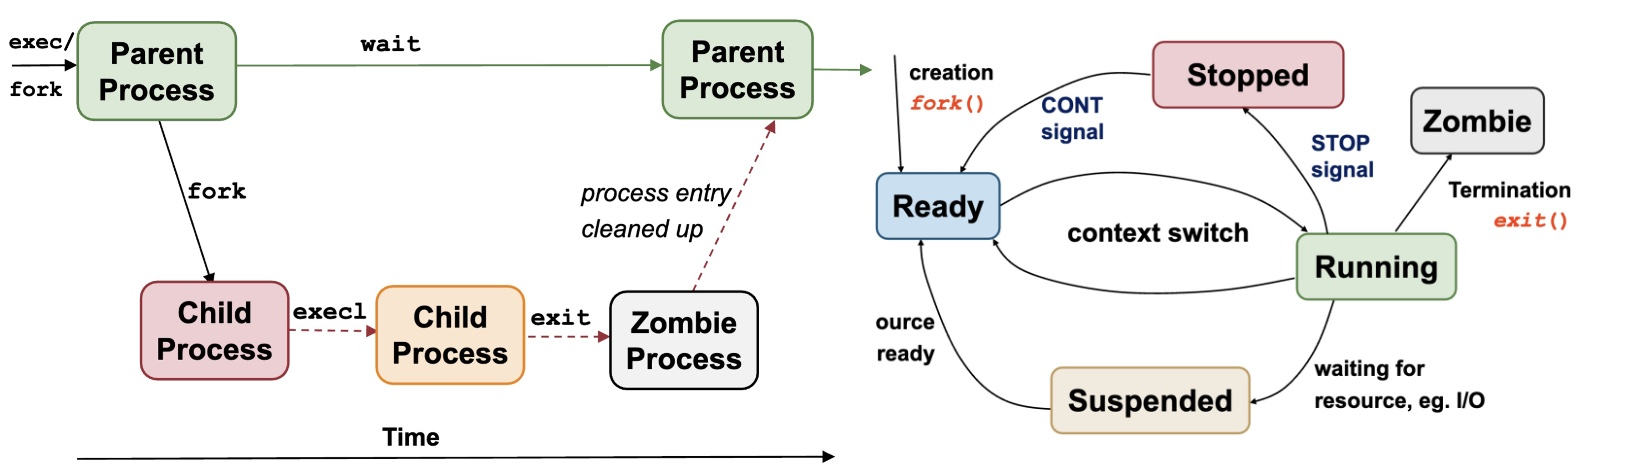
\includegraphics[
    width=\columnwidth,
    trim=0 0 0 0,
    clip
  ]{pro.jpg}%
}
\noindent\makebox[\columnwidth][c]{%
  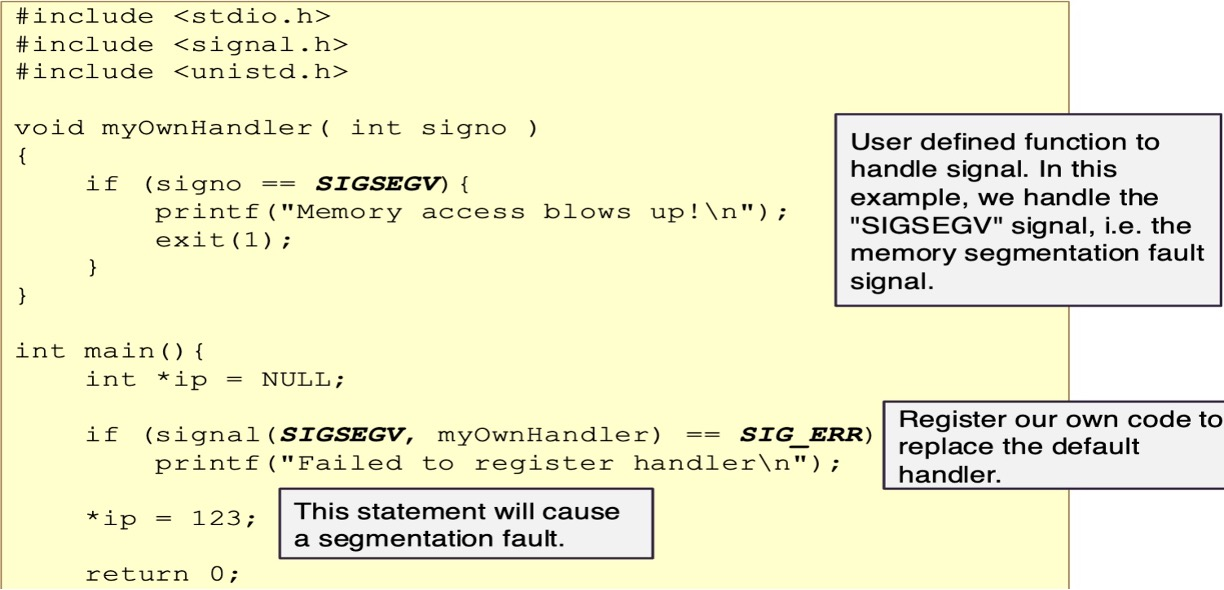
\includegraphics[
    width=\columnwidth,
    trim=0 0 0 0,
    clip
  ]{sig.jpg}%
}
\noindent\makebox[\columnwidth][c]{%
  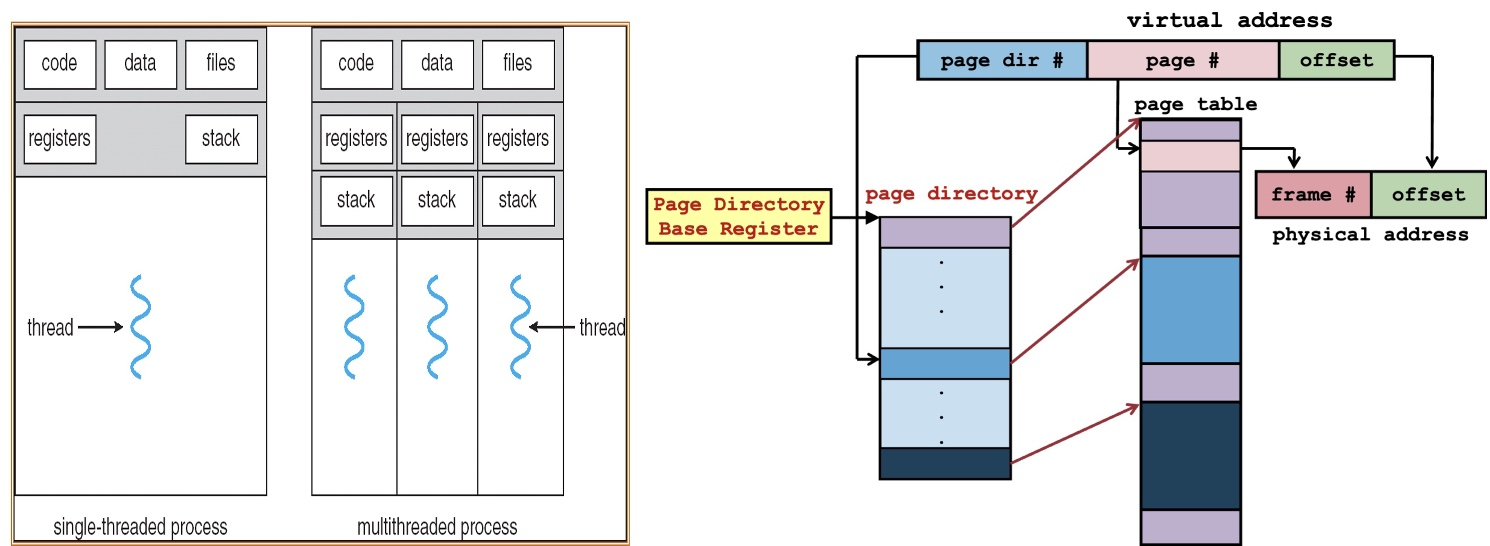
\includegraphics[
    width=\columnwidth,
    trim=0 0 0 0,
    clip
  ]{v.jpg}%
}
\noindent\makebox[\columnwidth][c]{%
  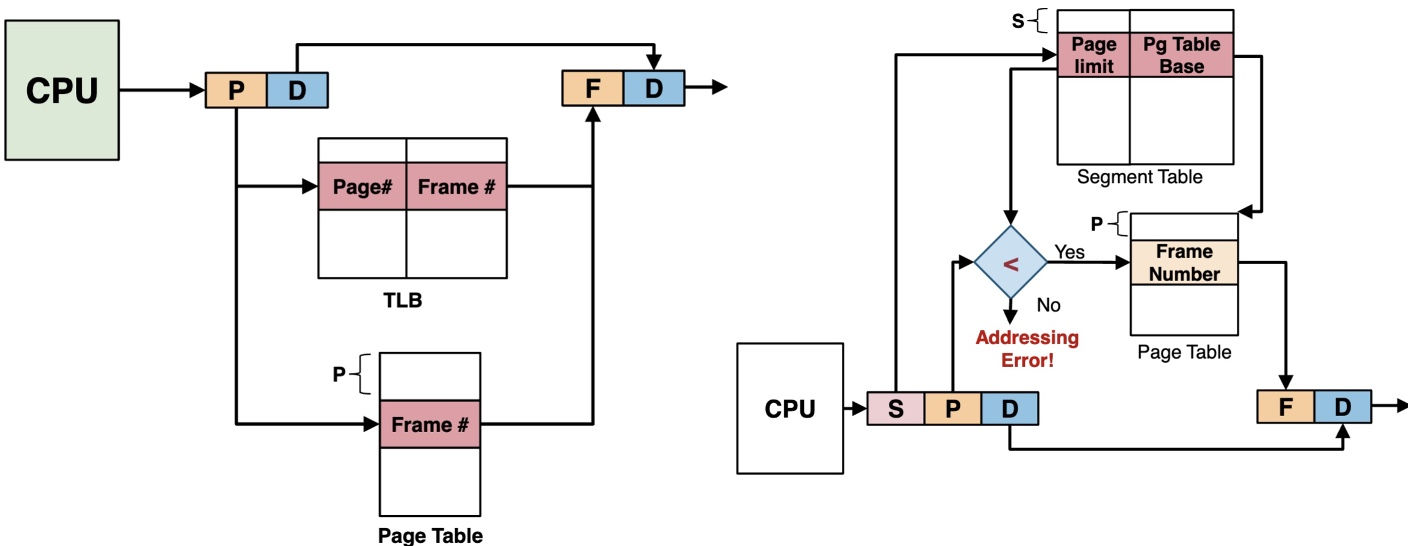
\includegraphics[
    width=\columnwidth,
    trim=0 0 0 0,
    clip
  ]{hd.jpg}%
}
\noindent\makebox[\columnwidth][c]{%
  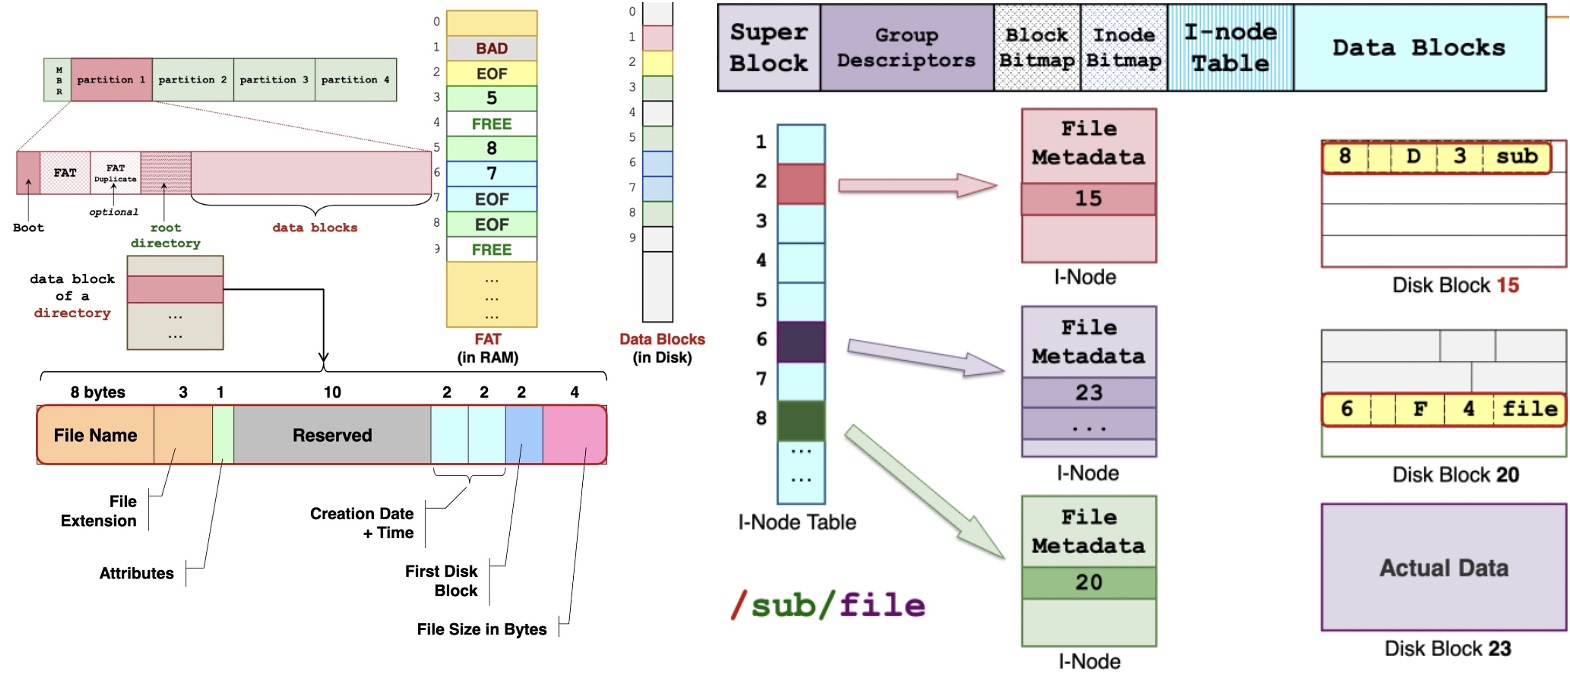
\includegraphics[
    width=\columnwidth,
    trim=0 0 0 0,
    clip
  ]{FATEXT.jpg}%
}
\noindent\makebox[\columnwidth][c]{%
  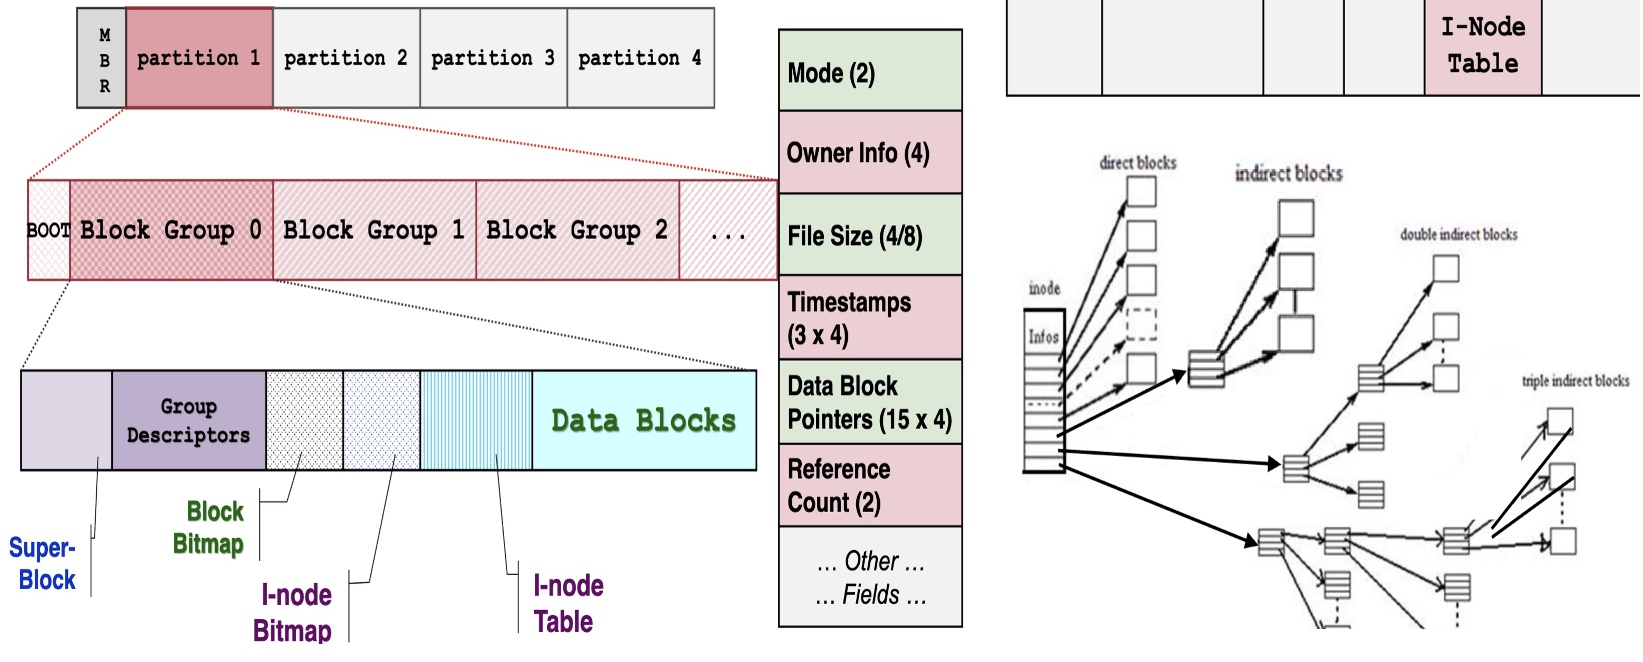
\includegraphics[
    width=\columnwidth,
    trim=0 0 0 0,
    clip
  ]{ext2.jpg}%
}
\noindent\makebox[\columnwidth][c]{%
  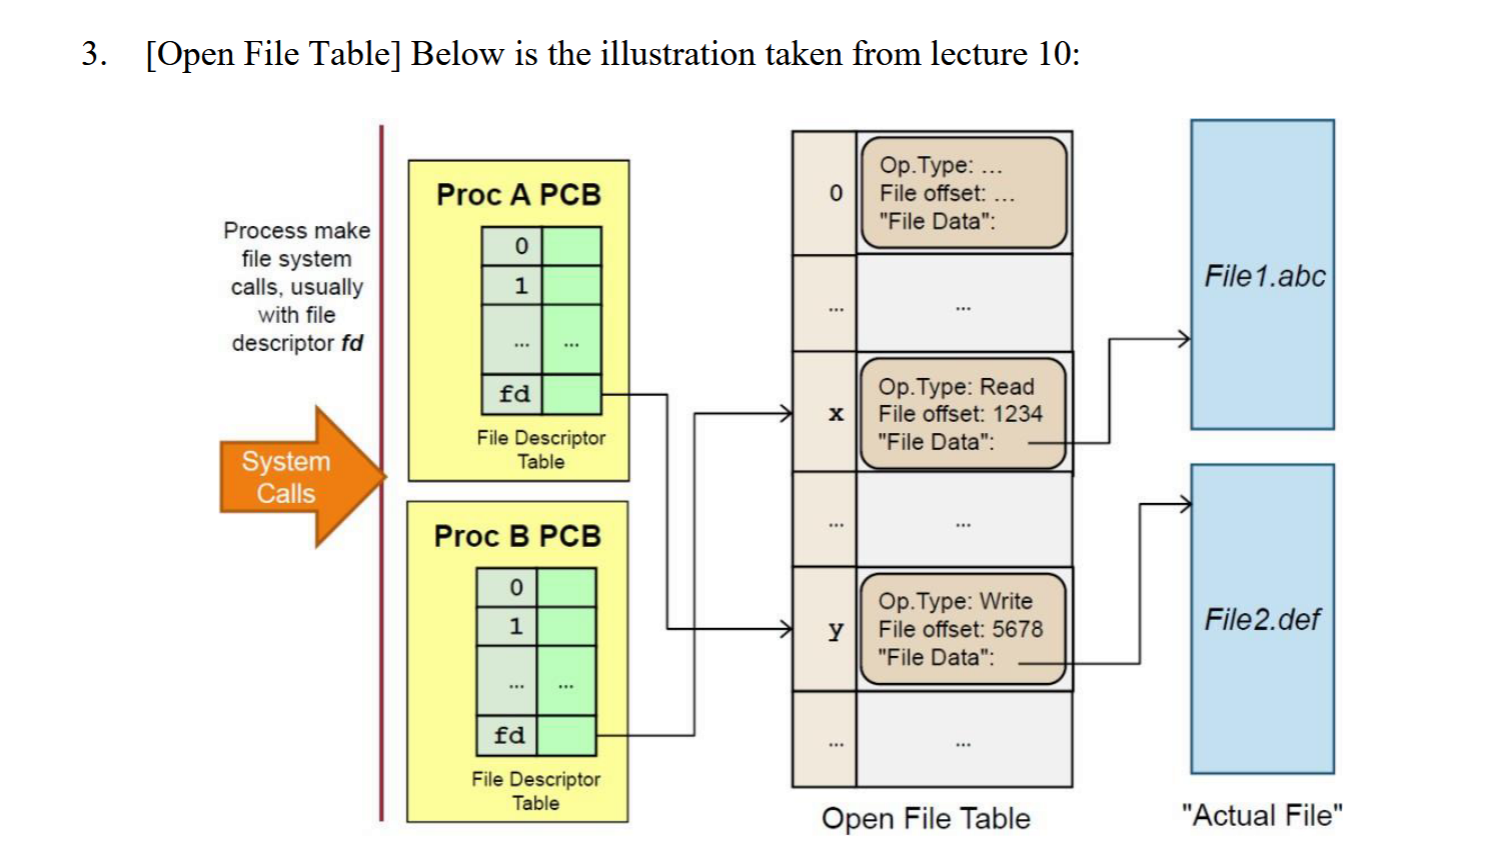
\includegraphics[
    width=\columnwidth,
    trim=0 0 0 0,
    clip
  ]{fd.png}%
}
\end{document}
